\chapter{Results}
\label{chapter:results}

We need some sort of tool to measure the ``goodness'' of the 
clustering. As we work with text data the dimensionality increases 
quite high and projecting data down to 2 or 3 dimensions for 
visualization is not a simple task. (We come back to visualization 
later though.)
So we have to resort to measurements derived from the 
resulting clustering itself. If we knew some underlying ground 
truth behind our clustering problem, we could validate our result 
against it. But as mentioned earlier, even defining what actually 
are the current fields of science depends on who you ask and for 
what purpose the definition is needed. So the ground truth is only
one measure for our results here.
In the lack of ground truth we can use some ``internal'' goodness 
measure for the resulting clustering. These kind of measures 
basically try to infer how dense the clusters are compared with how 
sparse the inter-cluster space is and how well the clusters are 
separated from each other.


\section{Silhouettes}
One such measure to estimate the ``goodness'' of a clustering is 
silhouettes. Silhouettes use average proximities which are know 
to work best with clear, compact and spherical clusters 
\cite{rousseeuw_silhouettes:_1987}. Silhouette value for an item 
is defined as:

Silhoutte values for 6000 publications clustered with 
agglomerative clustering with Ward's method, number of clusters 
64, are seen in Figure~\ref{fig:silh01}.
\begin{figure}[ht]
  \begin{center}    
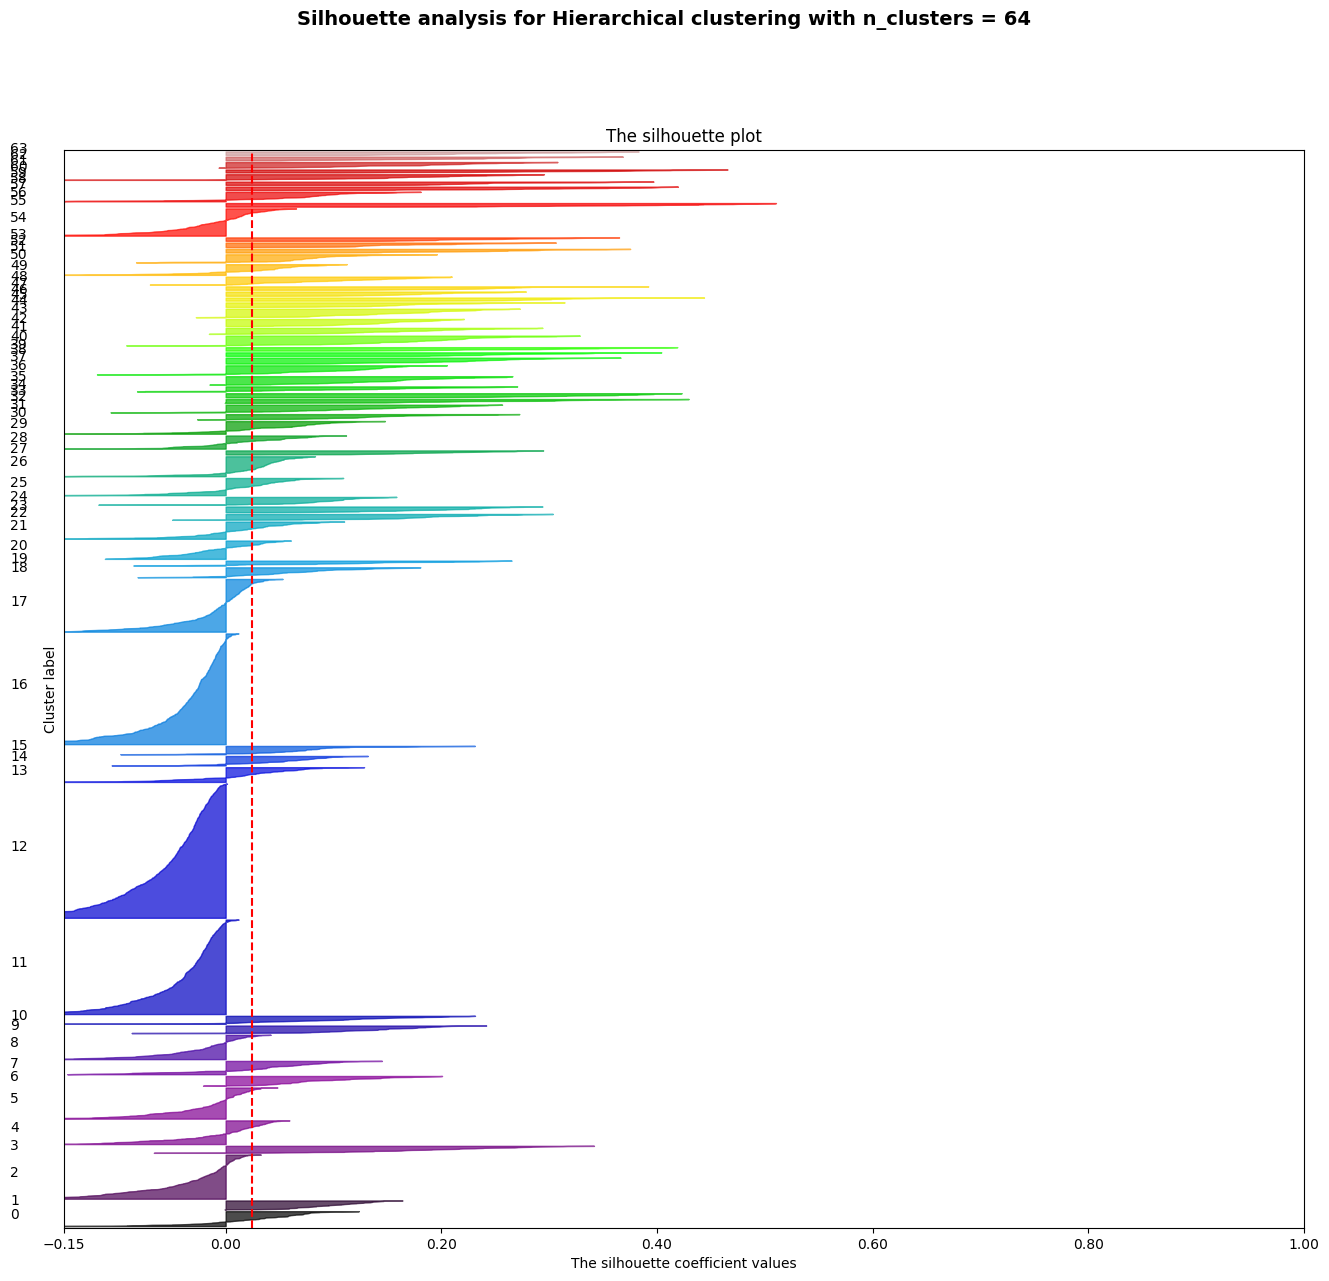
\includegraphics[width=13cm]{images/6000-64-400-Hierarchical-silhouette-plot.png}
    \caption{Silhoutte values of 6000 items clustered with 
    agglomerative clustering with Wrad's method, 64 clusters, 
    LSA with 400 components. Each pixel row corresponds to a 
    Silhouette value of an item, adjacent rows separated by gap 
    corresponds to a cluster.
    Dashed line is the average.}
    \label{fig:silh01}
  \end{center}
\end{figure}

Other measure is Calinski-Harabaz index. Clustering should be 
optimal when Calinski-Harabaz index reaches its maximum value. 
\cite{}

When evaluating the results, Silhouette Coefficient might not be
the best option. Find out why. V-measure or Adjusted Rand Index
might be better options \cite{noauthor_clustering_nodate}.


\section{``Gold standard set''}
We evaluated our clustering by creating an evaluation set with
hand labeled or verified fields of science. This subset of data 
consisted of 519 publications from three different fields. The fields
were: \emph{Computer science: Information systems}, 147 publications,
\emph{Computer science: Artificial intelligence} 153 publications, 
and \emph{Clinical neurology} 250 publications as classified by 
publisher. We checked the publisher labeling, \fixme{cleared the 
bad samples} lacking enough meta data, being too far out of the 
scope of any of the three disciplines or having corrupted data and
relabeled few \fixme{(amount)} samples to the more fitting 
discipline and to one discipline for each sample only. The ground 
truth labeling for 37 the most ambiguous samples was checked by 
a non-expert human reviewer. So, our manual classification will
be subjective but gives some hint about the classifier performance.
\fixme{Then we calculated precision and recall for the data set.} 

The Figure \ref{fig:ch-silh01} shows the results. We see that
Calinski-Harabasz index reaches it's maximum value at the number
of clusters two and that silhouette values increases with the
number of clusters.
Neither of these indices corresponds to the three disciplines
that we selected manually. It's also worth to remember that there
is only 519 data points to cluster. Comparison against preferred
manual labeling \fixme{is calculated with the 
Adjusted Rand Index (ARI) for these clusterings in Figure 
\ref{refhere}.}
Top terms for maximum index values are shown in the Table 
\ref{refhere}.

In figure \ref{fig:ch-silh02}
we see corresponding graphs for k-means clustering. Top terms for
Calinski-Harabasz index maximum at seven clusters are listed in 
the Table \ref{table:topterms}.


\begin{figure}[ht]
  \begin{center}    
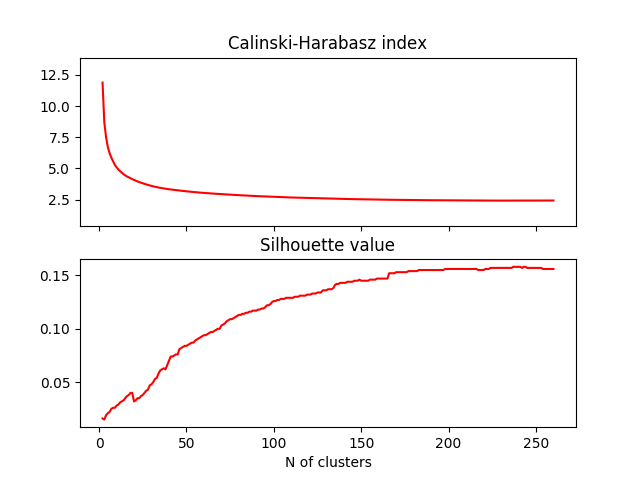
\includegraphics[width=9.5cm]{images/c-h-silh-index-plot-519-2_260-800-hierarchical.png}
    \caption{Hierarchical clustering. Calinski-Harabasz index and Silhoutte values for the
    manually annotated set of 519 publications clustered with hierarchical
    clustering, LSA with 800 components. The higher values denote 
    more compact and better clustering in both graphs.}
    \label{fig:ch-silh01}
  \end{center}
\end{figure}


\begin{figure}[ht]
  \begin{center}    
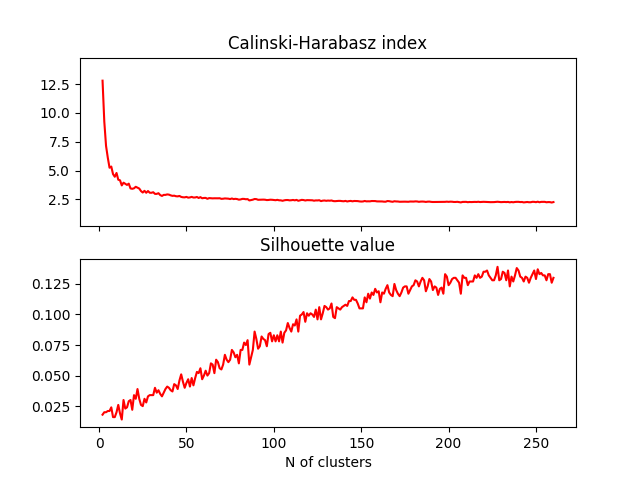
\includegraphics[width=9.5cm]{images/c-h-silh-index-plot-519-2_260-800-kmeans.png}
    \caption{k-means clustering. Calinski-Harabasz index and Silhoutte values for the
    manually annotated set of 519 publications clustered with k-means 
    clustering, LSA with 800 components. The higher values denote 
    more compact and better clustering in both graphs.}
    \label{fig:ch-silh02}
  \end{center}
\end{figure}

\begin{table}
\begin{tabular}{|p{2cm}|p{10.5cm}|} 
% Alignment of sells: l=left, c=center, r=right. 
% If you want wrapping lines, use p{width} exact cell widths.
% If you want vertical lines between columns, write | above between the letters
% Horizontal lines are generated with the \hline command:
\hline % The line on top of the table
\textbf{ } & \textbf{Top terms} \\ 
\hline 
\textbf{Cluster 0} & system internet management user project software architecture support decision business channel rule concept quality exercise  \\ 
\hline
\hline 
\textbf{Cluster 1} & lenges professional care intellectual disability people service special syndrome life child social support diagnosis pathology  \\ 
\hline
\hline 
\textbf{Cluster 2} & epilepsy stroke child seizure headache neuronal p rat sleep nerve risk treatment cell alcohol activity  \\ 
\hline
\hline 
\textbf{Cluster 3} & component filter signal neural linear bayesian ica feature value input simulation independent fuzzy vector output \\ 
\hline
\hline 
\textbf{Cluster 4} & dementia vascular ad cognitive stroke alzheimer diagnosis lesion vad risk pd brain impairment parkinson aneurysm \\ 
\hline
\hline 
\textbf{Cluster 5} & service development mobile switch agent system solution traffic environment protocol ip technology wireless game implementation \\ 
\hline
\hline 
\textbf{Cluster 6} & map image som self-organizing query logic document tree k expressive compression database retrieval rule cluster \\ 
\hline
\end{tabular} % for really simple tables, you can just use tabular
% You can place the caption either below (like here) or above the table
\caption{Top terms per cluster for manually annotated samples}
% Place the label just after the caption to make the link work
\label{table:topterms}
\end{table} % table makes a floating object with a title
cluster


\subsection{Precision and recall}
Recall is the number of items correctly classified divided by the 
total number of items in that class.
\begin{equation}
 Recall = \frac{|\{relevant\ items\} \cap \{retrieved\ items\}|} 
{\{relevant\ items\}}
\end{equation}
Precision is the number of items correctly classified divided by 
the total number items classified into that class (ie. true and 
false positives).
\begin{equation}
 Precision = \frac{|\{relevant\ items\} \cap \{retrieved\ 
items\}|} 
{\{retrieved\ items\}}
\end{equation}


\subsection{Other metrics}
Different metrics to evaluate clustering include (from 
scikit-learn) Adjusted Rand Index, Mutual Information scores 
(NMI, AMI), homogenity, completness, V-measure, Fowlkes-Mallows 
scores, Silhouette Coefficient, Calinski-Harabaz Index, (from 
sources) 


\section{Finnish publications from year 2000}
We clustered year 2000 data, 10145 publications, with k-means 
clustering with different value of $k$, the number of clusters. 
The Figure \ref{fig:ch-silh02} shows the results.
\begin{figure}[ht]
  \begin{center}    
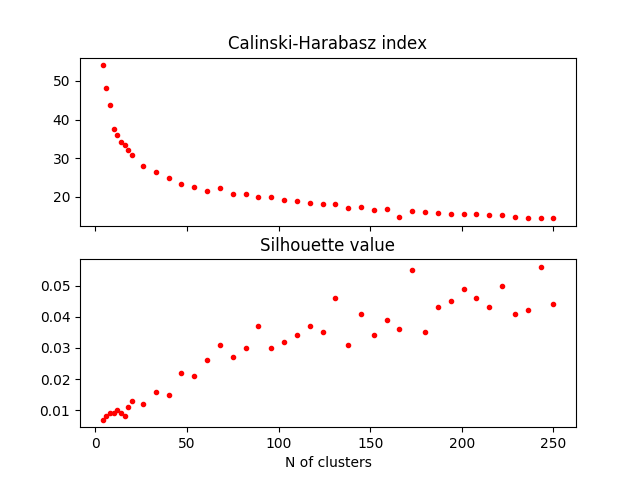
\includegraphics[width=10cm]{images/c-h-silh-index-plot-y2000-2_260-800-kmeans.png}
    \caption{Calinski-Harabasz index and Silhoutte values of 
10145 items clustered with k-means clustering, LSA with 800 
components. The higher values denote more compact and better 
clustering in both graphs.}
    \label{fig:ch-silh02}
  \end{center}
\end{figure}

Similarly the same data was clustered with agglomerative 
hierarchical Ward's clustering by sampling the number of clusters 
from the values [2-260]. The silhouette and Calinski-Harabasz values
are shown in Figure \ref{}
\begin{figure}[ht]
  \begin{center}    
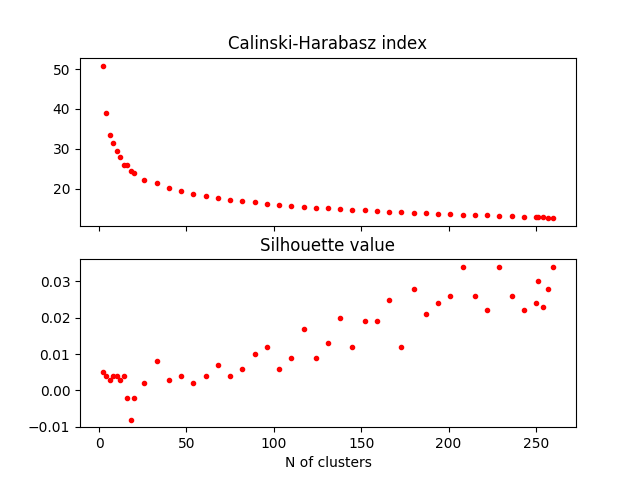
\includegraphics[width=10cm]{images/c-h-silh-index-plot-y2000-2_260-800-hierarchical.png}
    \caption{Hierarchical clustering. Calinski-Harabasz index and Silhoutte values for the
    Finnish publications from year 2000 clustered with hierarchical
    clustering, LSA with 800 components. The higher values denote 
    more compact and better clustering in both graphs.}
    \label{fig:ch-silh-2000-01}
  \end{center}
\end{figure}
We can see from the values that they prefer different features in
the data. Calinski-Harabasz index sees the fewest number of 
clusters - two - as the most compact and optimal clustering. Also
the form of the curve hints to perhaps power law that is also 
known as Zipf's law in text analysis. \fixme{Check this.}
It should be noticed that the silhouette values are quite low 
in absolute terms considering it's index space [-1,1]. This might 
be in line with the fact that it's best suited for [normally?] 
distributed and compact clusters. But we can also see that the 
silhouette values grow with the number of clusters although no
maxima seems to be reached with these cluster values.










